\documentclass[11pt]{article}
\usepackage[a4paper, portrait, margin=1in]{geometry}
\usepackage{hyperref}
% Fancy header package for version number

\usepackage{amsmath}
\usepackage{graphicx}
\usepackage{float}

\usepackage{fancyhdr}
\pagestyle{fancy}
\fancyhf{}
\renewcommand{\headrulewidth}{0pt}
\renewcommand{\footrulewidth}{0pt}
\newcommand{\Mod}[1]{\ (\text{mod}\ #1)}

\fancypagestyle{firstpagefooter}
{
\lfoot{Version: 29.09.2016}
\cfoot{}
\rfoot{\thepage}
}
\cfoot{\thepage}

\begin{document}

\title{Advanced Systems Lab (Fall'16) -- First
Milestone}

\author{\textbf{Name: \emph{Jo\~{a}o Louren\c{c}o Ribeiro}}\\\textbf{Legi number: \emph{15-927-999}}}

\date{
\vspace{4cm}
\textbf{Grading} \\
\begin{tabular}{|c|c|}
\hline  \textbf{Section} & \textbf{Points} \\
\hline  1.1 &  \\ 
\hline  1.2 &  \\ 
\hline  1.3 &  \\ 
\hline  1.4 &  \\ 
\hline  2.1 &  \\ 
\hline  2.2 &  \\ 
\hline  3.1 &  \\ 
\hline  3.2 &  \\ 
\hline  3.3 &  \\ 
\hline \hline Total & \\
\hline 
\end{tabular} 
}

\maketitle
\thispagestyle{firstpagefooter}
\newpage

\section{System Description}\label{sec:system-description}

\subsection{Overall Architecture}\label{sec:desc:architecture}

In this subsection, I provide an explanation of how the abstract architecture provided in the course has been implemented in terms of concrete classes, and outline the main design decisions. 

There is a main asynchronous receiving thread, which is an instance of the \texttt{Middleware} class\footnote{\url{https://gitlab.inf.ethz.ch/ljoao/asl-fall16-project/blob/master/src/joao/asl/Middleware.java}}. This thread is responsible for accepting connections from clients, as well as receiving incoming requests and processing them, i.e. routing them to the correct read queues (for \texttt{get} requests) or write queues (for \texttt{delete} and \texttt{set} requests). At a high level, it operates in a continuous \texttt{while} loop, constantly switching between looking for accept and read events from incoming connections, and processing the resulting requests. The reason to let the main receiving thread also process the requests is mainly one of consistency: if two \texttt{set} requests with the same key were sent to two different threads for processing, it could happen that their order would be swapped, which is undesirable. The main receiving thread has access to read and write queues, one of each per memcached server. This thread is also responsible for setting the time at which a request is received from a client, $T_{\textnormal{start}}$, and the time at which the request is enqueued, $T_{\textnormal{enqueued}}$.

The read/write queues are implemented as instances of \texttt{LinkedBlockingQueue}, which ensure thread safety, with the default maximum size (at most $2^{31}-1$ elements allowed in the queue simultaneously). These act essentially like unbounded queues, since it would be extremely unlikely to accumulate so many elements in a queue while the middleware is running. They are queues of instances of the \texttt{RequestSocketPair} class\footnote{\url{https://gitlab.inf.ethz.ch/ljoao/asl-fall16-project/blob/master/src/joao/asl/RequestSocketPair.java}}. Such an object is a pair with a request and the socket connecting to the respective client, so that the read and write threads know where to forward responses to later on.

The request/socket pairs in a queue are processed either by synchronous read threads (instances of the \texttt{ReadThread} class\footnote{\url{https://gitlab.inf.ethz.ch/ljoao/asl-fall16-project/blob/master/src/joao/asl/ReadThread.java}}) if they are \texttt{get} requests, or by asynchronous write threads (instances of the \texttt{WriteThread} class\footnote{\url{https://gitlab.inf.ethz.ch/ljoao/asl-fall16-project/blob/master/src/joao/asl/WriteThread.java}}), if they are \texttt{delete} or \texttt{set} requests. The \texttt{delete} requests are routed to write threads so that replicas of the stored value are also deleted. Each memcached server has an associated write thread, along with a read thread pool (an instance of the \texttt{ThreadPool} class\footnote{\url{https://gitlab.inf.ethz.ch/ljoao/asl-fall16-project/blob/master/src/joao/asl/ThreadPool.java}}), i.e. a collection of read threads with access to a common read queue. The details of the implementation of write threads, thread pools and read threads are discussed in Sections \ref{sec:desc:writes} and \ref{sec:desc:reads}. Finally, read and write threads are responsible for setting the time of dequeueing, $T_{\textnormal{dequeue}}$, the time a request is sent to the respective server(s), $T_{\textnormal{toserver}}$, the time the response is received from the server(s), $T_{\textnormal{fromserver}}$, the time the response is forwarded back to the client, $T_{\textnormal{end}}$, as well as the success flag of the request.

A diagram with the instants at which such timestamps are set in the flow of a request through the middleware can be found in Figure~\ref{diag}.

\begin{figure}[H]
	\centering
	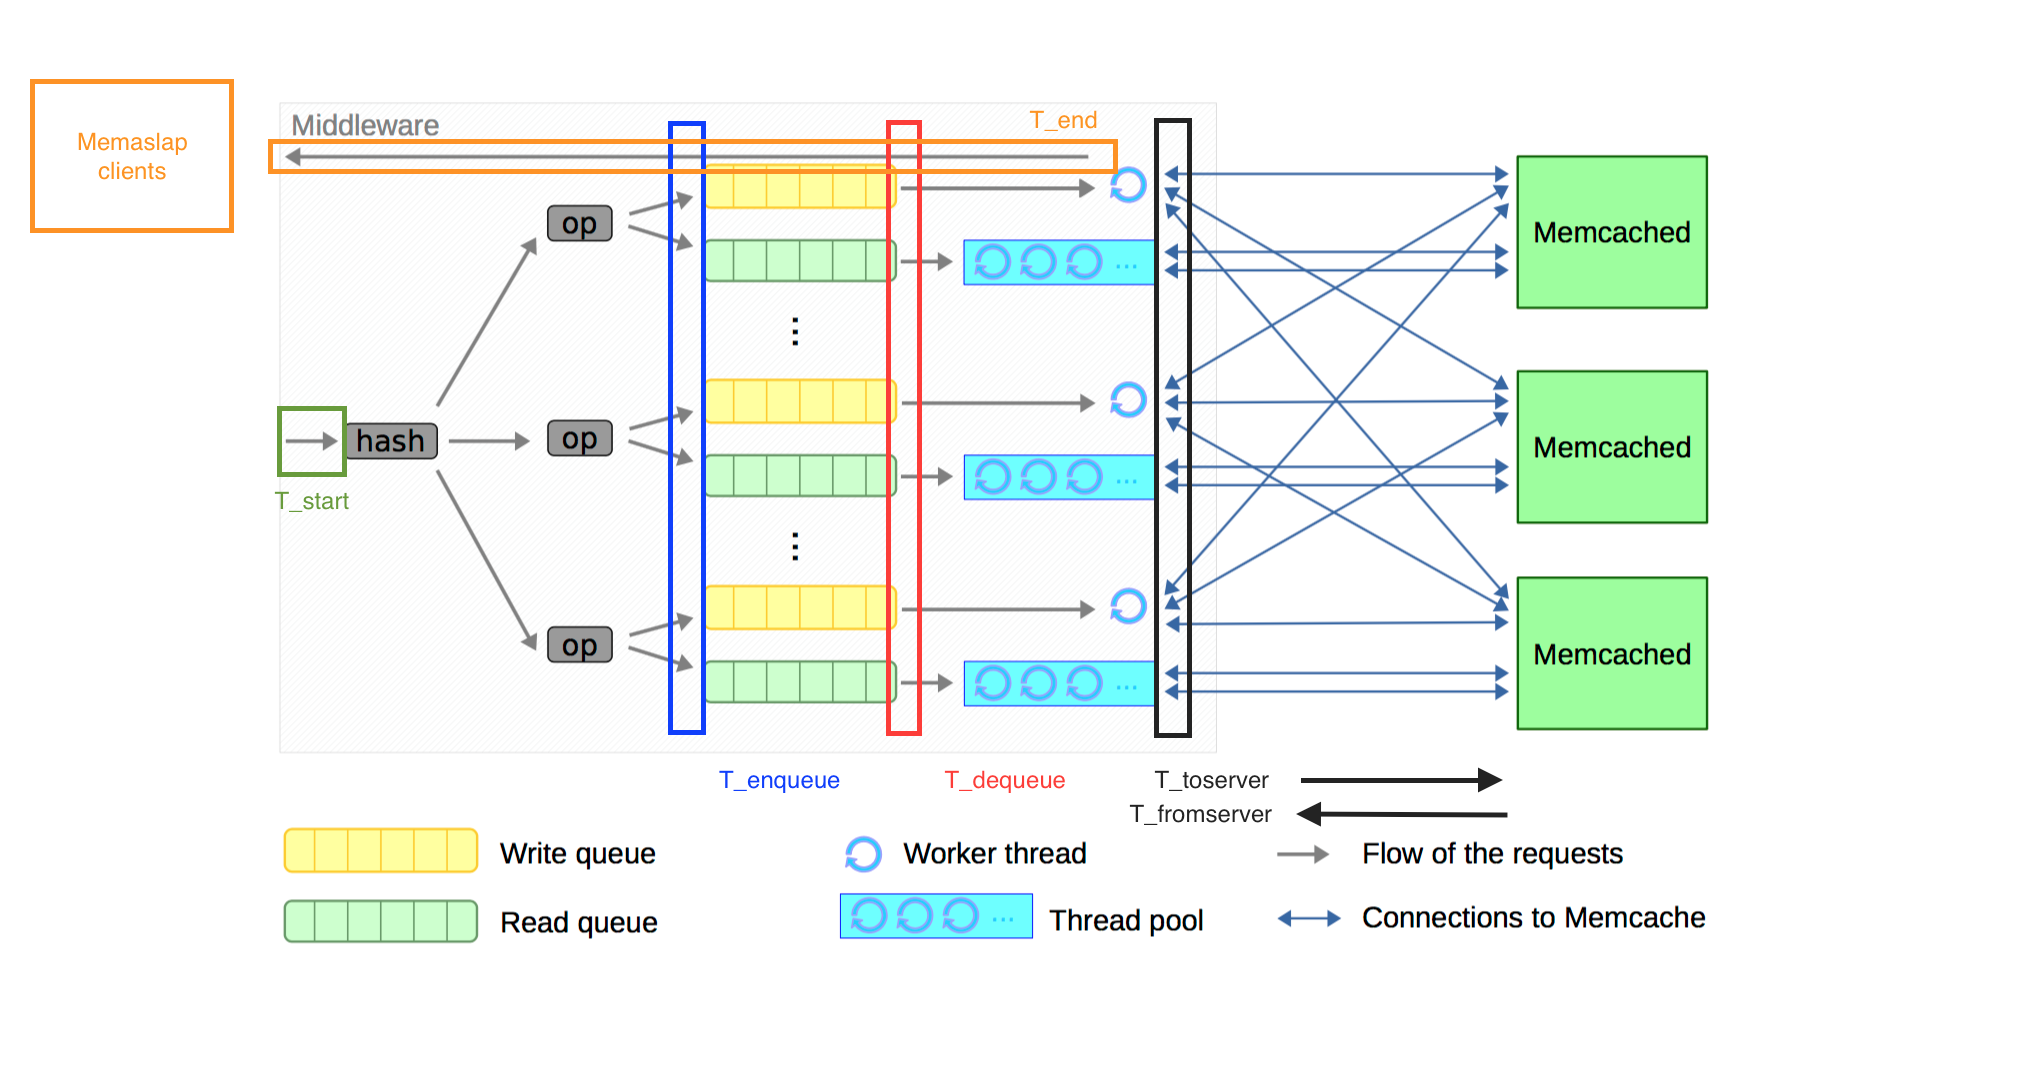
\includegraphics[width=0.9\textwidth]{abstract_arch_with_marks}
	\caption{An abstract diagram of the middleware architecture showing where all timestamps are recorded.}
	\label{diag}
\end{figure}

%Length: at most 1 page
%
%Explain how the abstract architecture we provided for you has been implemented in terms of classes and shortly outline the main design decisions. Mark on the figure where are the points that you instrumented the architecture (see Section~2.3 of the Project Description) and give the different timestamps a name that you\textbf{ will use throughout the three milestones }whenever referencing measurements (e.g., $T_{requestreceived}$, $T_{responsesent}$).
%
%Reference throughout the report all relevant java source files, result files, etc. by providing the gitlab link in a footnote, for instance\footnote{\url{https://gitlab.inf.ethz.ch/zistvan/asl-fall16-project/blob/master/src/ch/ethz/SomeClass.java}}. An exception to this rule is the referencing of log files belonging to experiments. These should be referenced by an ID, or short name, and there has to be a table at the end of the report mapping these to files in the git repository.

\subsection{Load Balancing and Hashing}\label{sec:desc:hashing}

The main receiving thread is responsible for accepting incoming connections, receiving requests from clients and routing them to the correct queues. This thread has a non-blocking instance of \texttt{ServerSocketChannel} registered for accept events. Each accepted connection leads to the creation of a non-blocking instance of \texttt{SocketChannel} from which the request is read and to where the response from memcached should be sent back. In order to correctly route this request, the thread extracts its operation and key. The corresponding server is then chosen by applying a hash function to the key, and the correct queue is chosen based on the operation type. One of the main objectives of the middleware is to ensure the requests are distributed over the servers as uniformly as possible. 

To ensure close-to-uniform load balancing, the middleware uses the following hash function: when given a string $x$ of length 16, it applies the \texttt{hashCode()} method of the \texttt{String} class, and then mods the result with respect to the total number of servers, say $n$. The output of this procedure is thus $y=x.\texttt{hashCode()}\Mod{n}\in\{0,\dots,n-1\}$. If the servers are given as input to the middleware in the order $\textnormal{server}_0,\dots,\textnormal{server}_{n-1}$, where $\textnormal{server}_i$ represents the IP address and port of the $i$th server given to the middleware, then the request associated with $x$ is routed to $\textnormal{server}_y$. Furthermore, if the replication factor is $r$, the neighbors of $\textnormal{server}_k$ are $\textnormal{server}_{k+1 \Mod n},\dots,\textnormal{server}_{k+r-1\Mod n}$. Every set request sent to $\textnormal{server}_k$ is also written into its neighbors.

Assuming a uniform distribution over 16-byte keys, the \texttt{hashCode()} method aims to provide a close-to-uniform distribution over 32-bit signed integers for use in clustering\footnote{\url{https://en.wikipedia.org/wiki/Java_hashCode()}}. Furthermore, if the distribution induced by applying \texttt{hashCode()} to 16-byte keys is indeed almost uniform, then applying $\Mod{n}$ afterwards, for any $n$, again induces an almost uniform distribution over $\{0,\dots,n-1\}$.

To further support the short reasoning of the last paragraph, I ran a small experiment. For $n=2,\dots, 7$ (representing the number of servers), the following is repeated five times: generate 100.000 strings of length 16 uniformly at random, then compute their hashes and count how many strings are assigned to each server. The number of strings generated is chosen to be 100.000 because it is a decently-sized lower bound estimate on the number of \texttt{set} requests received in a long run of the middleware. To measure how close the induced distribution is to a uniform distribution, I compute the statistical distance between them for every repetition, and then take the maximum over the five values. The statistical distance of a random variable $X$ over $\{0,\dots,n-1\}$ to a uniform distribution over the same set is given by
\[
	d(X)=\frac{1}{2}\sum_{i=0}^{n-1}\left|\Pr[X=i]-\frac{1}{n}\right|.
\]
If $d(X)=\delta$, then $|\Pr[X=i]-1/n|\leq \delta$ for every $i$. Thus, a value of $d(X)$ close to 0 indicates that the distribution induced by the observed frequency counts is close-to-uniform. The statistical distances obtained in the experiment are summarized in the table below, rounded up to 4 decimal places. The code used in the experience can be found in gitlab\footnote{\url{https://gitlab.inf.ethz.ch/ljoao/asl-fall16-project/blob/master/hash_test/HashTest.java}}.

\small{
	\smallskip
	\begin{tabular}{|c|c|}
		\hline Number of servers & Max. Statistical Distance (out of 5 repetitions) \\ 
		\hline 2 & 0.0011 \\ 
		\hline 3 & 0.0025 \\ 
		\hline 4 & 0.0030 \\
		\hline 5 & 0.0044 \\ 
		\hline 6 & 0.0050 \\ 
		\hline 7 & 0.0044 \\
		\hline
	\end{tabular} }\\

Given the results of the experiment, I can conclude that the induced distributions are almost uniform. In fact, the observed frequencies were always within 0.5\% of the probabilities given by the relevant uniform distributions. Thus, the proposed hash function achieves its goal of close-to-uniform load balancing.

\subsection{Write Operations and Replication}\label{sec:desc:writes}

In order to handle write operations and replication, each server has an associated write thread, which is an instance of the \texttt{WriteThread} class. This thread has access to a write queue (an instance of \texttt{LinkedBlockingQueue}) containing pairs of requests and associated sockets, which are instances of \texttt{RequestSocketPair}. The request/socket pairs are put in the queue by the main receiving thread of the middleware through the \texttt{put()} method.

Write threads are asynchronous, and function in a continuous while loop. First, the thread checks whether the write queue is non-empty. If yes, it removes the head of the queue and sets $T_{\textnormal{dequeue}}$. Then, it extracts the relevant request, and forwards it to the primary server and its $r-1$ neighbors, where $r$ is the replication factor. After the first write (which is to the primary server), it sets $T_{\textnormal{toserver}}$, and continues writing to the remaining servers (the neighbors). The write thread keeps $r$ non-blocking \texttt{SocketChannel} instances permanently open while the middleware is running, each connected to one of the primary server and its neighbors. These sockets are registered for read events in a selector. After a request is forwarded to all relevant servers, it is added to a queue of sent requests, which is an instance of \texttt{LinkedList} whose elements are strings.

If the write queue is empty, the thread skips the steps above and proceeds directly to checking for read events from its sockets. This is done by invoking the \texttt{selectNow()} method and then iterating over all the ready events. When processing such an event, the thread reads from the relevant sockets and splits the array obtained into the (perhaps several) responses contained in it. Then, for each response, it sets $T_{\textnormal{fromserver}}$ and creates an instance of the \texttt{ResponseTimePair} class\footnote{\url{https://gitlab.inf.ethz.ch/ljoao/asl-fall16-project/blob/master/src/joao/asl/ResponseTimePair.java}} containing a response and the respective time (this time coincides for all the responses that arise from the same array). The write thread contains, for each associated server, a queue of responses, which is an instance of \texttt{LinkedList} whose elements are instances of \texttt{ResponseTimePair}. The response/time pairs read from a given server are added into the associated queue.

Lastly, the thread checks whether all the response queues are non-empty. If yes, then the head responses of each queue are exactly the responses to the head request of the queue of sent requests. Thus, the thread removes the request and the corresponding responses, and checks whether they were all successful. If yes, then it sets the success flag to true, sets $T_{\textnormal{fromserver}}$ as the maximum over the timestamps of all the responses, forwards the response back to the client, and finally sets $T_{\textnormal{end}}$. If some response is an error, then the thread forwards the error to the client and sets the timestamps as described, but leaves the success flag as false. If some of the response queues are empty, then the thread goes back to checking for new requests in the write queue.

The replicated case differs from the ``write one" scenario only on the number of response queues in the write thread, and also the number of servers it writes to.

The factors which I believe limit the rate at which writes can be carried are five. First, the quality of the client-middleware and middleware-server connections, since a transmission rate limit in such connections implies immediately a hard lower bound on the response time. Second, the specifications of the machine which runs the middleware limits the speed at which the write thread can cycle through the loop and process write requests. Third, the number of read threads affects the rate, since they steal computing time from the write threads. Fourth, the minimum response time for the memcached server itself also gives a hard lower bound on the response time for write requests. Lastly, the replication factor limits the rate as well, since it increases the number of total threads in the middleware and forces the response time to depend on the performance of several servers.

%Length: at most 1 page
%
%Provide a short description of how the writes are handled in the middleware. Explain how the replicated case differs from the simple ``write one'' scenario. 
%
%Give an estimate of the latencies the writing operation will incur, and generalize it to the replicated case. What do you expect will limit the rate at which writes can be carried out in the system (if anything)?

\subsection{Read Operations and Thread Pool}\label{sec:desc:reads}

To handle read operations, each server has an associated thread pool, which is an instance of the \texttt{ThreadPool} class. A thread pool consists of a collection of read threads that share access to a common queue of pairs of read requests and associated sockets (instances of \texttt{RequestSocketPair}), which, as previously mentioned, is an instance of \texttt{LinkedBlockingQueue}. Each read thread is an instance of the \texttt{ReadThread} class. The request/socket pairs are put in the queue by the main receiving thread of the middleware through the \texttt{put()} method, and then are removed by the read threads in the thread pool using the \texttt{take()} method. Note that \texttt{LinkedBlockingQueue} is a queue implementation found in the \texttt{java.util.concurrent} package, and so it is thread-safe\footnote{\url{https://docs.oracle.com/javase/7/docs/api/java/util/concurrent/BlockingQueue.html}}. The \texttt{take()} method for dequeueing is thread-safe and ensures that each read thread blocks while waiting for the read queue to be non-empty. Thus, no problems arise from several read threads accessing the same read queue in parallel.

Each read thread in a thread pool has a blocking instance of \texttt{SocketChannel} which is connected to the associated memcached server. This socket is kept permanently open while the middleware is running. Thus, if a thread pool has $t$ threads, then it also has $t$ blocking sockets connected to the relevant memcached server.

After taking a request/socket pair from the queue, the read thread sets $T_{\textnormal{dequeue}}$. Then, it simply forwards the request to the memcached server through the blocking socket, and sets $T_{\textnormal{toserver}}$. Afterwards, it blocks waiting for the response from the server and sets $T_{\textnormal{fromserver}}$, and then forwards it to the client through the socket associated to the request. Finally, it sets $T_{\textnormal{end}}$ and logs the request if its log flag is set to \texttt{true}.

\section{Memcached Baselines}\label{sec:baseline}

In this section, the goal is to understand how memcached behaves as a function of the number of virtual clients connected to it in the Microsoft Azure cloud. In particular, it is of interest to understand how the average aggregated throughput and average response time of a memcached server scale as a function of the number of virtual clients which connect to it.

Each experiment consists of running two memaslap instances in parallel connected to the memcached server for one minute in the Azure cloud, with the settings mentioned in the paragraph below. For each given number of virtual clients, an experiment is repeated five times. The average aggregated throughput, average response time and its standard deviation are recorded for each experiment from the logs generated by memaslap. I decided to run each experiment for one minute instead of thirty seconds in order to better smooth out abnormal behavior, for example caused by the two memaslap instances not starting at the exact same time.

To run the experiments, consider three distinct Basic A2 Azure virtual machines in the same private network. One machine runs a memcached server with one thread, while the other two machines run one instance of memaslap each. The setup of the memaslap instances depends on the number of clients considered. I decided to vary this number from 4 to 128 in jumps of 4. I opted to distribute the number of virtual clients (i.e. the concurrency) evenly between the two memaslap instances, so as to avoid abnormal behavior produced by memaslap instances with different loads. Furthermore, the memcached server is restarted after each 1 minute run so that the increasing number of items in the server does not affect later experiments. The number of threads in a memaslap instance is always set to the same value as the concurrency. Furthermore, each instance is ran with \texttt{-o 0.9} and uses the \texttt{smallvalue} configuration file provided. A summarized version of the experimental setup can be found below. 

\small{
\smallskip
\begin{tabular}{|c|c|}
\hline Number of servers & 1 (Basic A2) \\ 
\hline Number of client machines & 2 (Basic A2) \\ 
\hline Virtual clients / machine & 2 to 64, increased in steps of 2 (evenly distributed) \\ 
\hline Workload & Key 16B, Value 128B, Writes 1\% (\texttt{smallvalue}) \\
\hline Overwrite (\texttt{-o}) & 0.9\\
\hline Middleware & Not present \\ 
\hline Runtime x repetitions & 1m x 5 \\ 
\hline 
\end{tabular} }\\

%This section will report experimental results. All such parts will start with a short description of the experimental setup. The log files should be identified by a short name, or number, which will be explicitly listed at the end of the document (see Logfile Listing at the end).  \textbf{If this table is missing or the logfiles listed can't be found in your repository the experiment could be considered invalid, and no points will be awarded!}
%For baseline measurement of memcached provide \textbf{two} graphs (Section~\ref{sec:baseline:tput} and \ref{sec:baseline:rt}), one with aggregated throughput and one with average response time and standard deviation as a function of number of virtual clients. Increase these in steps from 1 to 128. Give a short explanation of memcache's behavior and find the number of virtual clients that saturate the server.
%
%\small{
%\smallskip
%\begin{tabular}{|c|c|}
%\hline Number of servers & 1 \\ 
%\hline Number of client machines & 1 to 2 \\ 
%\hline Virtual clients / machine & 1 to 64 \\ 
%\hline Workload & Key 16B, Value 128B, Writes 1\% \footnotemark \\
%\hline Middleware & Not present \\ 
%\hline Runtime x repetitions & 30s x 5 \\ 
%\hline Log files & microbench1, microbench2, \ldots \\
%\hline 
%\end{tabular} }
%
%\footnotetext{As starting point use the workloads provided in \url{http://www.systems.ethz.ch/sites/default/files/file/asl2016/memaslap-workloads.tar}. Use by default the \emph{small} workload. In later experiments you can and should change read-write ratios and potentially use other value sizes.}




\subsection{Throughput}\label{sec:baseline:tput}

The average aggregated throughput of each repetition can be found in baseline-tps1, baseline-tps2, baseline-tps3, baseline-tps4 and baseline-tps5, parameterized by the number of virtual clients. The average over the five repetitions for each number of virtual clients can be found in baseline-tps, and its plot can be found in Figure~\ref{baseline:tps}.

\begin{figure}[H]
	\centering
	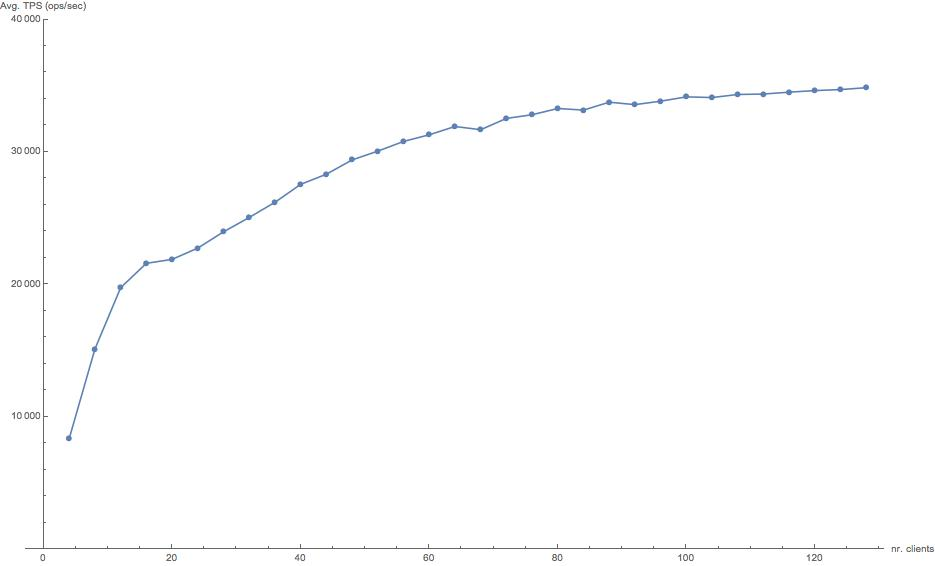
\includegraphics[width=0.9\textwidth]{baseline_tps}
	\caption{Average aggregated throughput per number of virtual clients. The plotted values can be found in baseline-tps. The data from each repetition can be found in baseline-tps1 through baseline-tps5.}
	\label{baseline:tps}
\end{figure}

Looking at the plot of Figure \ref{baseline:tps}, one notices that throughput increases steeply at first and then the slope of the curve decreases, becoming almost constant when the load (number of requests per second) imposed on the server approaches its load limit. In fact, as expected, the resulting curve resembles a ``real" throughput curve as shown in the tutorial, except for some mismatches which do not detract from its interpretation. I also conclude that the server becomes saturated at the 88 clients mark, for the reasons showcased next. This (88 clients) is a point where the slope increases slightly and then returns to its pattern of decrease. Note that the absolute difference in aggregated throughput between consecutive points after the 88 clients mark only goes above 260 ops/sec once (from 96 to 100), and it stays well below this value most of the time. On the other hand, the throughput difference between consecutive points before the 88 clients mark is generally much larger, even as we get closer to this value, where we witness differences of about 400-600 ops/sec (e.g. 76 to 80 and 84 to 88).

%First, at the 20 clients mark, the slope decreases remarkably and then increases again immediately, continuing its pattern of steady decrease from there on. Second, at the 68, 80 and 88 clients marks there seem to be bumps that fall very slightly outside the observable trend of the curve.

\subsection{Response time}\label{sec:baseline:rt}

The average response time and standard deviation of each repetition can be found in baseline-avg1, baseline-avg2, baseline-avg3, baseline-avg4 and baseline-avg5, parameterized by the number of virtual clients. The average over the five repetitions (for both response time and standard deviation) for each number of virtual clients can be found in baseline-avg, and its plot can be found in Figure~\ref{baseline:avg}. While the average of the standard deviations does not yield the standard deviation of the response time over the 5 repetitions and the 2 clients, it does provide an upper bound on this value. Furthermore, it also showcases the expected standard deviation of response time of a client during a single run of the experiment, which is an important parameter.

\begin{figure}[H]
	\centering
	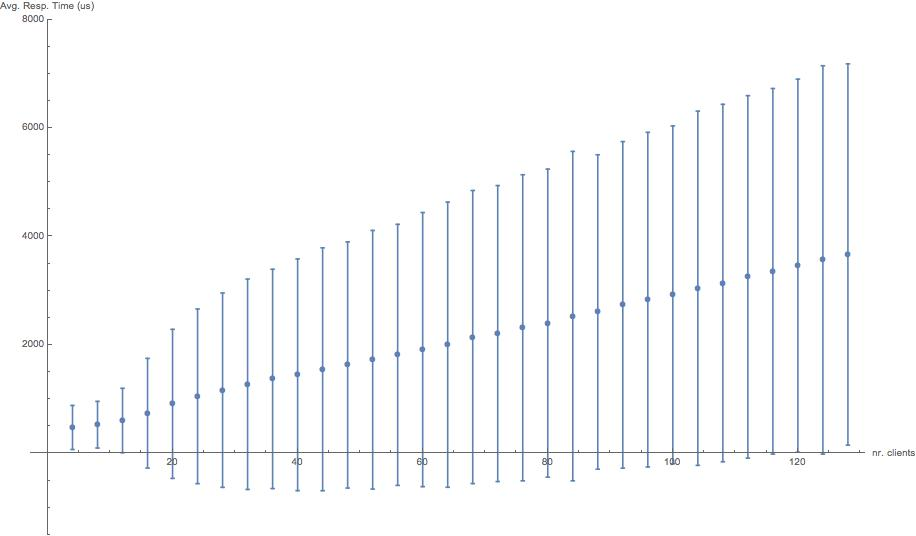
\includegraphics[width=0.9\textwidth]{baseline_avg}
	\caption{Average response time (in microseconds) and standard deviation per number of virtual clients. Plotted values can be found in baseline-avg-std. The data from each repetition can be found in baseline-avg-std1 through baseline-avg-std5.}
	\label{baseline:avg}
\end{figure}

First, note that an increase in the number of virtual clients implies a larger load of requests being continuously sent to the server. This means that the server has to deal with a larger amount of requests continuously throughout the experiment, and thus average response time should increase in general. Furthermore, more virtual clients means a larger number of connections between the memaslap instances and the server. Since these are established between different machines in a network and not locally, their performance is much less stable. This leads to a higher variance in response times around the mean, as transmission rates in the connections can fluctuate unpredictably during the experiment. Thus, such instability contributes both to an increase in average response time and to an increase in standard deviation, which explains the observations.

\section{Stability Trace}\label{sec:trace}

The goal of this section is to show that the middleware is functional and can handle workload for an extended amount of time without degrading in performance in the Microsoft Azure cloud. I decided to present two experiments with different sampling methods (1 second sampling and 10 seconds sampling in memaslap) in order to showcase a more complete picture of the performance of the middleware. The experimental setup can be summarized as follows: 

\small{
	\smallskip
	\begin{tabular}{|c|c|}
		\hline Number of servers & 3 (Basic A2) \\ 
		\hline Number of client machines & 3 (Basic A2) \\ 
		\hline Virtual clients / machine & 64 \\ 
		\hline Workload & Key 16B, Value 128B, Writes 1\% (\texttt{smallvalue}) \\
		\hline Overwrite (\texttt{-o}) & 0.9\\
		\hline Middleware & Present (Basic A4)\\ 
		\hline Threads in pool & 32\\
		\hline Replication & 3\\
		\hline Experience 1 & 1h x 1, \texttt{-S 1s} \\
		\hline Experience 2 & 1h x 1, \texttt{-S 10s} \\ 
		\hline
	\end{tabular} }\\

The throughput, average response time and standard deviation are recorded for each sample point provided by the memaslap instances. Afterwards, an 1 hour portion of these logs is plotted. In the next Sections, I present the relevant plots and respective log files, as well as explanations for the behavior observed.

The logs pertaining to each experiment conducted in this Section can be found in the caption of the respective plot.

\subsection{Throughput}\label{sec:tps}

In this section I present two 1 hour-long throughput plots from the setup previously described, pertaining to two different runs of the experiment. In the first run, memaslap instances sampled throughput every second (\texttt{-S 1s} in memaslap). In the second run, throughput is sampled over 10 seconds windows (\texttt{-S 10s} in memaslap). The first plot is featured in Figure~\ref{trace:tps1}, and the second plot in Figure~\ref{trace:tps10}. Explanations for the behavior observed can be found in Section~\ref{sec:overhead}. The relevant logs can be found in the descriptions of the figures.

\begin{figure}[H]
	\centering
	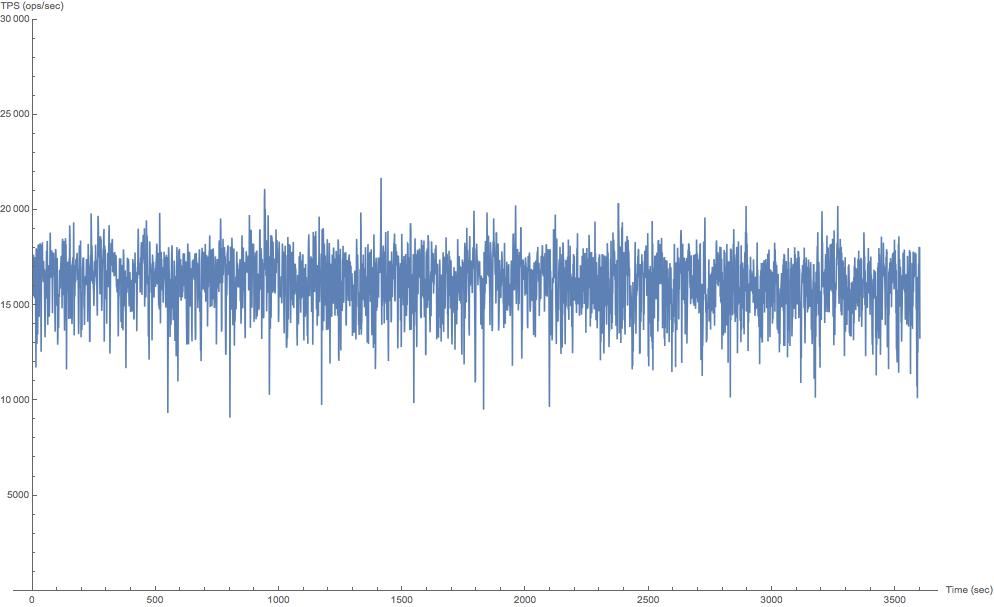
\includegraphics[width=0.9\textwidth]{trace_tps_1s_3600}
	\caption{Throughput as a function of time (in seconds), sampled for each 1 second window (\texttt{-S 1s} in memaslap), in a stability trace experiment. Plotted values can be found in trace1s-tps. The data from each client can be found in trace1s-tps1, trace1s-tps2 and trace1s-tps3.}
	\label{trace:tps1}
\end{figure}

\begin{figure}[H]
	\centering
	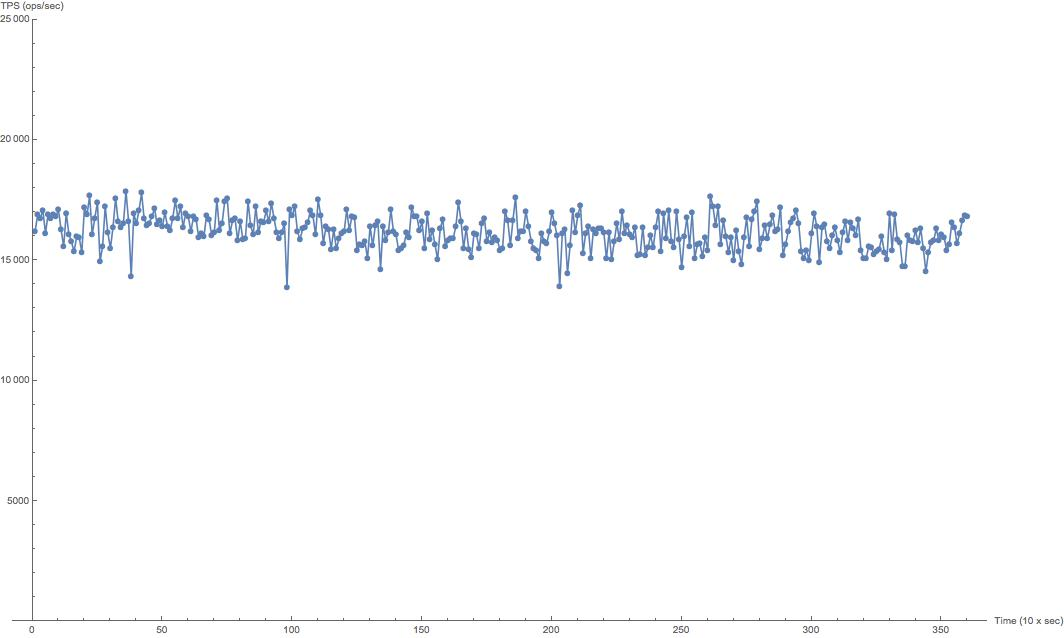
\includegraphics[width=0.9\textwidth]{trace_tps_10s_3600}
	\caption{Throughput as a function of time (in periods of 10 seconds), sampled and averaged over intervals of 10 seconds (\texttt{-S 10s} in memaslap), in a stability trace experiment. The plotted values can be found in trace10s-tps. The data from each client can be found in trace10s-tps1 through trace10s-tps3.}
	\label{trace:tps10}
\end{figure}

\subsection{Response time}\label{sec:avg}

In this section I present 1 hour-long average response time plots corresponding to the runs of the experiment described in Section 3.1. There are four plots in total. The first two (Figures \ref{trace:avg1} and \ref{trace:avg-std1}) correspond to the run of the first plot of Section~\ref{sec:tps} (Figure~\ref{trace:tps1}), where memaslap computes average response times and standard deviation over 1 second windows (\texttt{-S 1s} in memaslap). Of these two plots, the first features only average response time, while the second features average response time with standard deviations as error bars. The next two plots (Figures \ref{trace:avg10} and \ref{trace:avg-std10}) follow the same scheme, but pertain to the run where memaslap instances compute averages over windows of 10 seconds (\texttt{-S 10s} in memaslap), which corresponds also to the second throughput plot in Section~\ref{sec:tps} (Figure~\ref{trace:tps10}). Again, I present several plots both for clarity of presentation (it can be harder to read the average response time from plots that feature also the standard deviation) and to obtain a more complete picture of the performance of the middleware. Explanations for the behavior observed can be found in Section~\ref{sec:overhead}. As mentioned and justified in Section~\ref{sec:baseline:rt}, standard deviation is plotted as the average of the standard deviations of the 3 clients. Thus, one obtains the expected standard deviation of a client's response times during one run of the experiment, for each time interval sampled.

\begin{figure}[H]
	\centering
	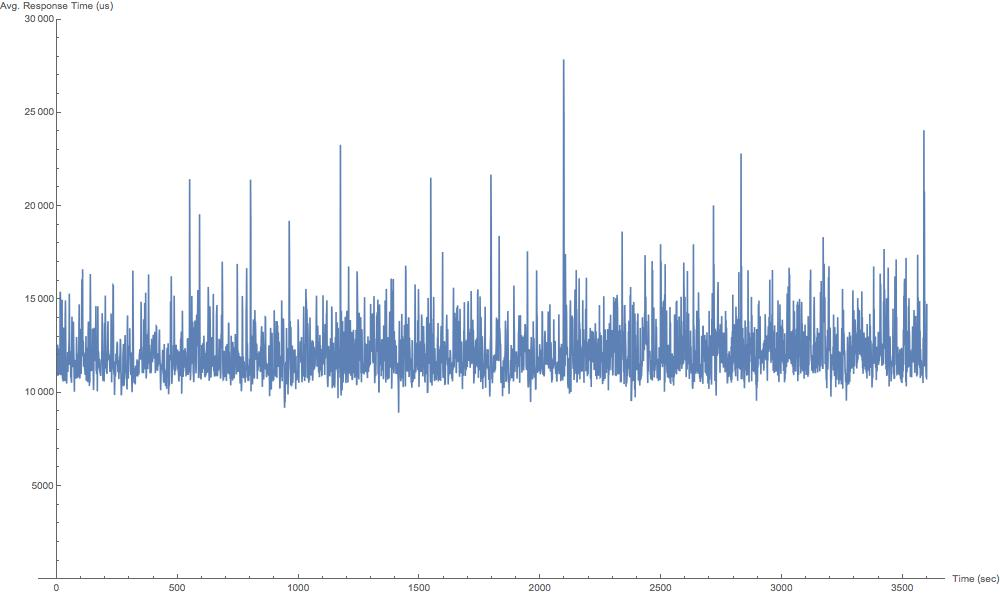
\includegraphics[width=0.9\textwidth]{trace_avg_1s_3600}
	\caption{Average response time (in microseconds) as a function of time (in seconds), computed for each 1 second window (\texttt{-S 1s} in memaslap), in a stability trace experiment. The plotted values can be found in trace1s-avg. The data from each client can be found in trace1s-avg1 through trace1s-avg3.}
	\label{trace:avg1}
\end{figure}

\begin{figure}[H]
	\centering
	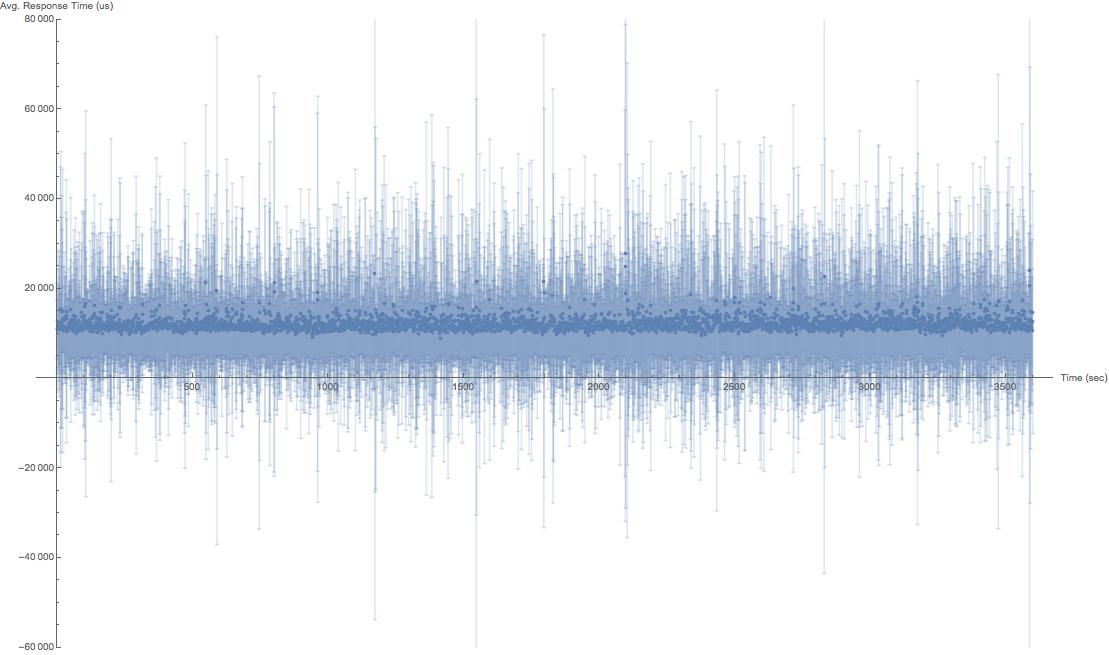
\includegraphics[width=0.9\textwidth]{trace_avg_std_1s_3600_clipped}
	\caption{Average response time (in microseconds) and standard deviation as functions of time (in seconds), computed for each 1 second window (\texttt{-S 1s} in memaslap), in a stability trace experiment. The plotted values can be found in trace1s-avg-std. The data from each client can be found in trace1s-avg-std1 through trace1s-avg-std3. Note that extreme outliers values for standard deviation are clipped for readability.}
	\label{trace:avg-std1}
\end{figure}

\begin{figure}[H]
	\centering
	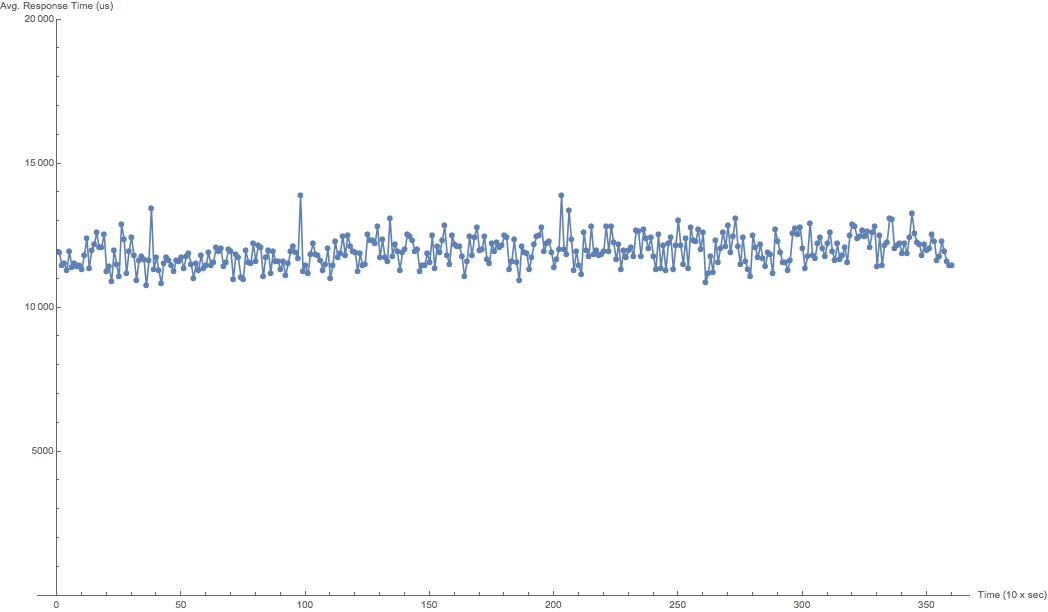
\includegraphics[width=0.9\textwidth]{trace_avg_10s_3600}
	\caption{Average response time (in microseconds) as a function of time (in periods of 10 seconds), computed for each 10 second window (\texttt{-S 10s} in memaslap), in a stability trace experiment. The plotted values can be found in trace10s-avg. The data from each client can be found in trace19s-avg1 through trace10s-avg3.}
	\label{trace:avg10}
\end{figure}

\begin{figure}[H]
	\centering
	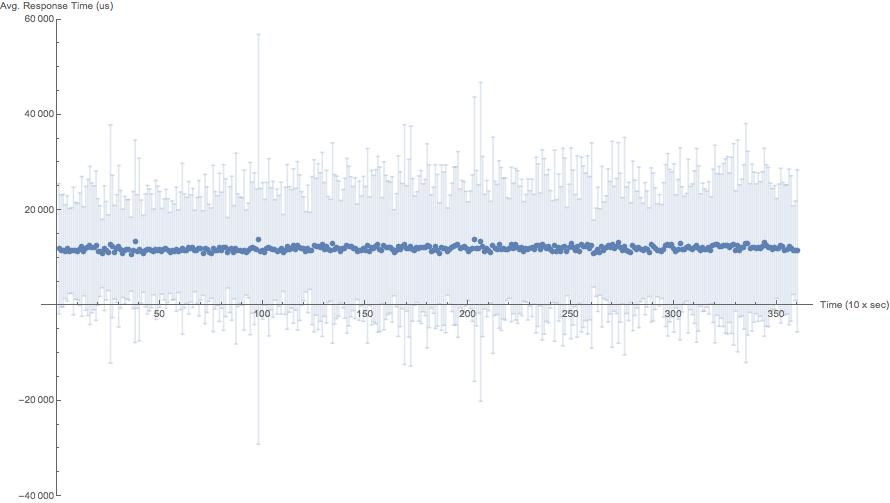
\includegraphics[width=0.9\textwidth]{trace_avg_std_10s_3600}
	\caption{Average response time (in microseconds, dark blue) and standard deviation (light blue) as functions of time (in periods of 10 seconds), computed for each 10 second window (\texttt{-S 10s} in memaslap), in a stability trace experiment. The plotted values can be found trace10s-avg-std. The data from each client can be found in trace10s-avg1 through trace10s-avg3.}
	\label{trace:avg-std10}
\end{figure}

\subsection{Overhead of middleware}\label{sec:overhead}

The goal of this section is twofold: first, to compare the expected performance of the middleware in the cloud with the one observed in Sections \ref{sec:tps} and \ref{sec:avg} based on the baselines, and attempt to explain the divergences. Second, to quantify the overhead that the middleware introduces over the baselines.

For all the figures found below, as mentioned and justified in Section~\ref{sec:baseline:rt}, standard deviation is plotted as the average of the standard deviations of the clients whenever applicable.

A prediction of the performance of the middleware in the cloud depends not only on the baseline experiments, but also on local stability traces with the same setup as the experiment in the cloud. First, Figures \ref{local:tps} and \ref{local:avg-std} show that the middleware performs consistently in terms of throughput and average response time when the 3 clients/ 3 servers/ full replication setup is run locally for 45 minutes. This experiment was performed in a MacBook Pro with 8GB of memory and a 2.6GHz Intel Core i5 processor. The experimental setup is summarized below.

\small{
	\smallskip
	\begin{tabular}{|c|c|}
		\hline Number of servers & 3 (Local) \\ 
		\hline Number of client machines & 3 (Local) \\ 
		\hline Virtual clients / machine & 64 \\ 
		\hline Workload & Key 16B, Value 128B, Writes 1\% (\texttt{smallvalue}) \\
		\hline Overwrite (\texttt{-o}) & 0.9\\
		\hline Middleware & Present (Local)\\ 
		\hline Threads in pool & 32\\
		\hline Replication & 3\\
		\hline Runtime x repetitions, sampling & 45m x 1, \texttt{-S 1s} \\
		\hline
	\end{tabular} }

\begin{figure}[H]
	\centering
	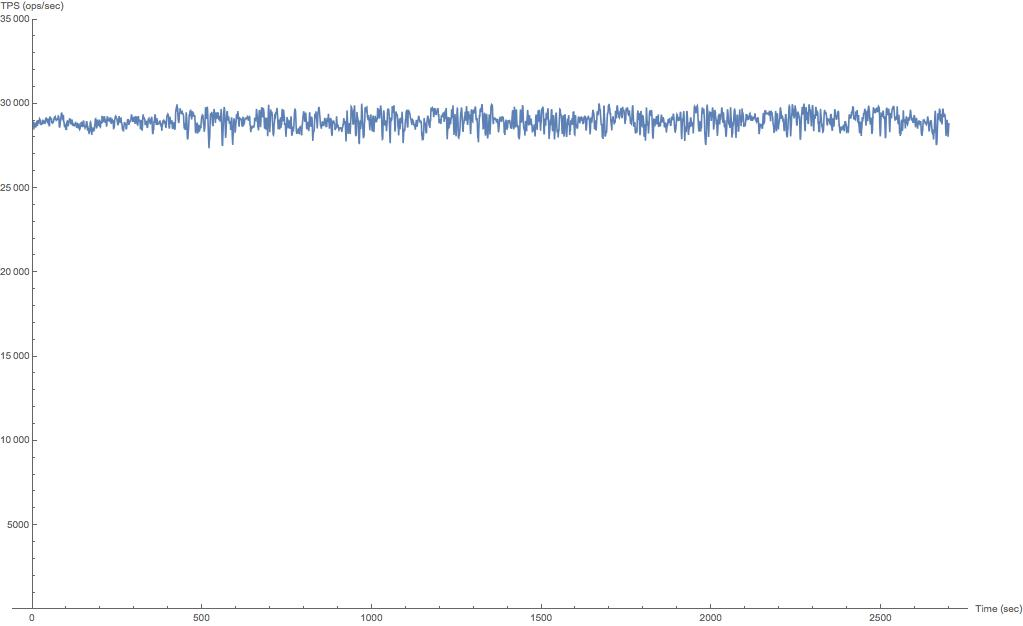
\includegraphics[width=0.9\textwidth]{local_tps_2700}
	\caption{Throughput as a function of time (in seconds), sampled for each 1 second window (\texttt{-S 1s} in memaslap), in a local stability trace. The plotted values can be found in local-tps. The data from each client can be found in local-tps1 through local-tps3.}
	\label{local:tps}
\end{figure}

\begin{figure}[H]
	\centering
	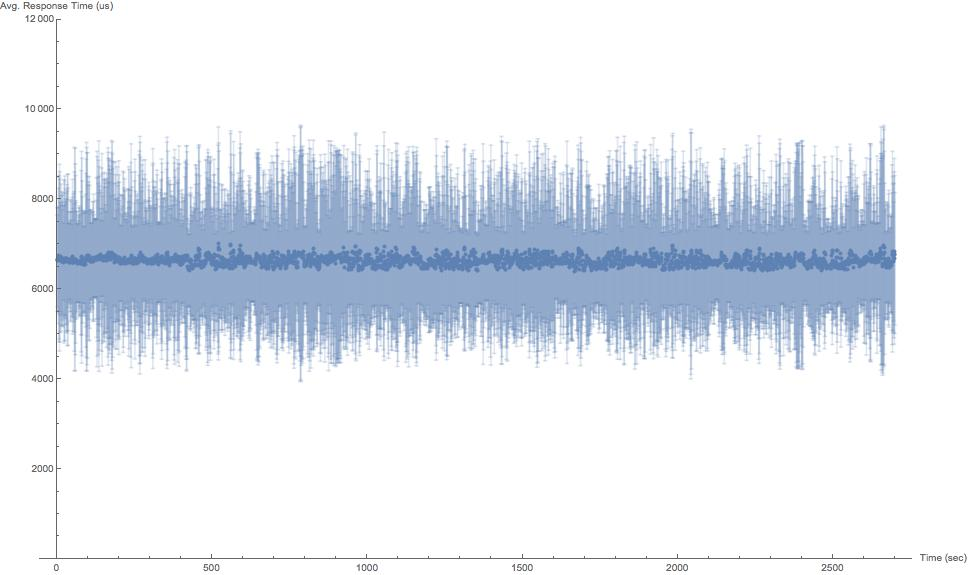
\includegraphics[width=0.9\textwidth]{local_avg_std_2700}
	\caption{Average response time (in microseconds, dark blue) and standard deviation (light blue) as functions of time (in seconds), computed for each 1 second window (\texttt{-S 1s} in memaslap), in a local stability trace. The plotted values can be found in local-avg-std. The data from each client can be found in local-avg-std1 through local-avg-std3.}
	\label{local:avg-std}
\end{figure}

The average response time plot from the baseline experiments (Figure~\ref{baseline:avg}) shows that the expected standard deviation of a client during a run of the experiment is roughly of the order of the average response time throughout the whole plot. While in the baseline experiment we only deal with two memaslap instances connected to a single memcached server, in the stability trace experiment we deal with three memaslap instances and three memcached servers, which are intermediately connected to the middleware. This means that the number of connections between machines in the cloud for the stability trace is much larger than for the baseline experiments. Furthermore, full replication introduces dependence between the connections from the middleware to the memcached servers, which further amplifies the effect of the connections between machines in the stability trace experiment. Lastly, requests still have to flow through the middleware, which adds some more variation to response times. Thus, I expected that the standard deviation would be somewhat larger than the average response time in the stability trace experiment in the cloud, in order to account for influences of the extra connections, their interdependence, and the middleware. This, in turn, would imply larger variation in average response time and consequently in throughput for the stability trace, especially when these values are measured every second.

Combining the local stability trace (Figures \ref{local:tps} and \ref{local:avg-std}), the baseline experiments and the remarks of the last paragraph, I expected that the middleware would achieve lower throughput and average response time during the stability trace experiment, with a standard deviation normally somewhat larger than the corresponding average response time (as mentioned above). Moreover, throughput and average response time would be subject to larger variations than the ones witnessed locally, since there would be an extra influence from the non-local connections between clients, middleware and servers, but would still be within sensible lower and upper limits in variation. Nevertheless, since the middleware produced a stable local trace, I expected that it would also produce a stable trace in the cloud,  in the sense that the size of the variation window for throughput and average response time would remain quite consistent throughout a 1 hour-long trace, especially when sampling over larger time intervals (e.g. 10 seconds instead of 1 second). Furthermore, I expected standard deviation to stay somewhat consistent throughout the trace when sampling over larger time intervals (e.g. 10 seconds instead of 1 second).

Observing the plots in Sections \ref{sec:tps} and \ref{sec:avg}, one can see that the predictions hold well, especially when throughput, average response time and standard deviation are computed over larger time intervals (Figures \ref{trace:tps10}, \ref{trace:avg10} and \ref{trace:avg-std10}). Nevertheless, there are noticeable and large (mainly downward for throughput, upward for response time) spikes in performance in the plots of the 1 second-interval stability trace (Figures \ref{trace:tps1}, \ref{trace:avg1} and \ref{trace:avg-std1}). Observing the plots of the 10 second-interval stability trace (Figures \ref{trace:tps10}, \ref{trace:avg10} and \ref{trace:avg-std10}), one notes that the spikes are smoothed out. This leads me to conclude that these are sudden and only momentary spikes. After such a spike occurs, the system returns immediately to more normal and expected behavior.

It remains to discover whether such spikes are a product of abnormal behavior of the middleware itself in the cloud, or if they are a result of instabilities in the cloud which are independent from the middleware. In order to find this out, I decided to run a single memaslap instance with 64 virtual clients and threads, \texttt{-o 0.9}, and using the \texttt{smallvalue} configuration file, connected to a memcached server in the cloud for at least 1 hour, without a middleware. The server and the client were in different virtual machines in the cloud, and memaslap recorded throughput, average response time and standard deviation every second (\texttt{-S 1s}). The experimental setup is summarized below.

\small{
	\smallskip
	\begin{tabular}{|c|c|}
		\hline Number of servers & 1 (Basic A2) \\ 
		\hline Number of client machines & 1 (Basic A2) \\ 
		\hline Virtual clients / machine & 64 \\ 
		\hline Workload & Key 16B, Value 128B, Writes 1\% (\texttt{smallvalue}) \\
		\hline Overwrite (\texttt{-o}) & 0.9\\
		\hline Middleware & Not present\\ 
		\hline Runtime x repetitions, sampling & 1h x 1, \texttt{-S 1s} \\
		\hline
	\end{tabular} }\\

The relevant plots can be found in Figures \ref{long:tps}, \ref{long:avg} and \ref{long:avg-std}. The values used in each of these plots can be found in the logs.

\begin{figure}[H]
	\centering
	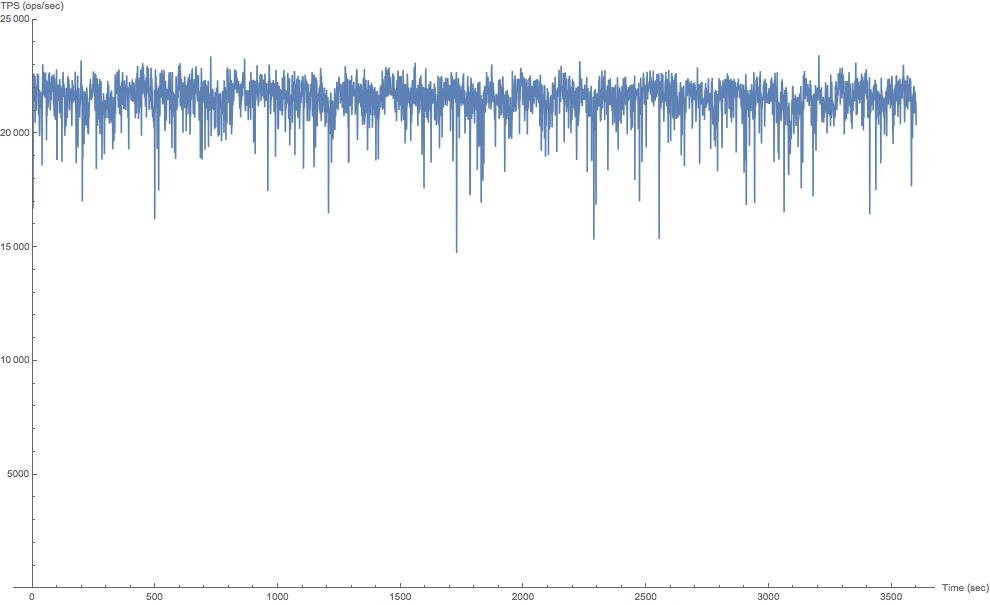
\includegraphics[width=0.9\textwidth]{baseline_tps_3600}
	\caption{Throughput as a function of time (in seconds), computed for each 1 second window (\texttt{-S 1s} in memaslap), in the stability trace for a 1 server/1 client/no middleware setup in the cloud. The plotted values can be found in no-mw-tps.}
	\label{long:tps}
\end{figure}

\begin{figure}[H]
	\centering
	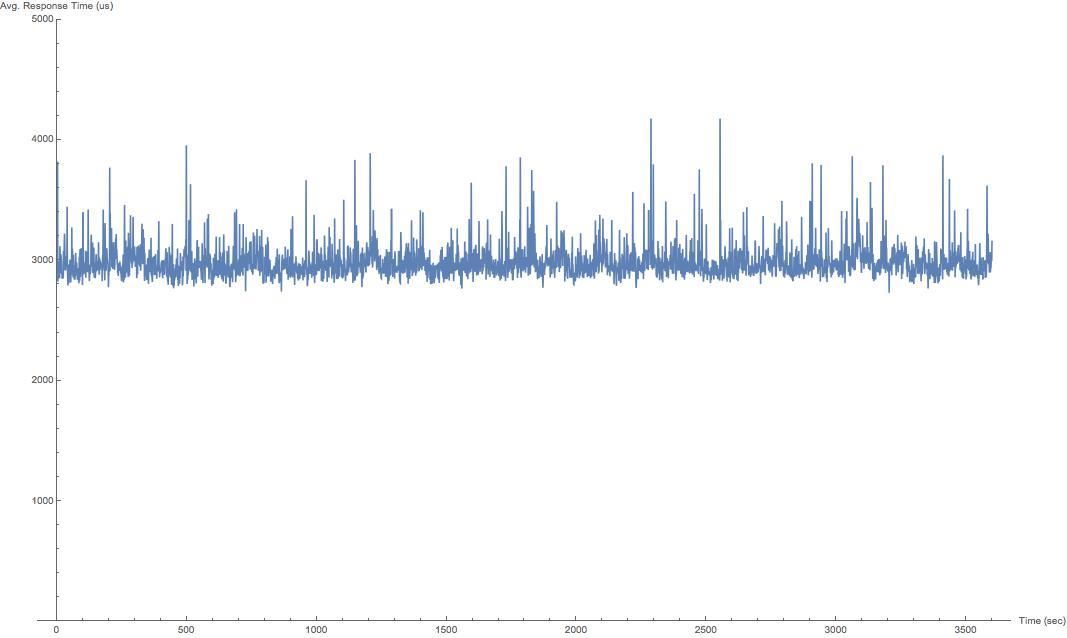
\includegraphics[width=0.9\textwidth]{baseline_avg_3600}
	\caption{Average response time (in microseconds) as a function of time (in seconds), computed for each 1 second window (\texttt{-S 1s} in memaslap), in the stability trace for a 1 server/1 client/no middleware setup in the cloud. The plotted values can be found in no-mw-avg.}
	\label{long:avg}
\end{figure}

\begin{figure}[h]
	\centering
	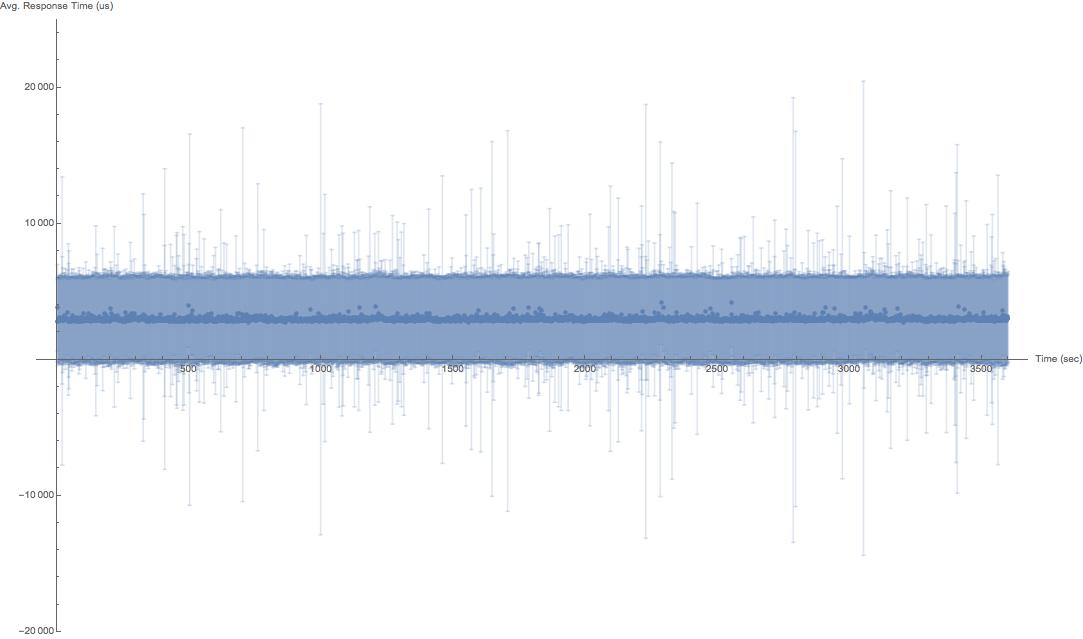
\includegraphics[width=0.9\textwidth]{baseline_avg_std_3600}
	\caption{Average response time (in microseconds, dark blue) and standard deviation (light blue) as functions of time (in seconds), computed for each 1 second window (\texttt{-S 1s} in memaslap), in the stability trace for a 1 server/1 client/no middleware setup in the cloud. The plotted values can be found in no-mw-avg-std.}
	\label{long:avg-std}
\end{figure}

Observing the plots of Figures \ref{long:tps}, \ref{long:avg} and \ref{long:avg-std}, it is clear that these have striking similarities with the plots of figures in Sections \ref{sec:tps} and \ref{sec:avg}, albeit with a smaller variation window for throughput and average response time. This is expected, since the current experiment features a much less complex situation, just 1 server and 1 client, as opposed to 3 servers, 3 clients, and a middleware with several threads and connections to servers. Most importantly, these plots still feature sudden spikes in performance, both in throughput and response time, which occur with very similar frequencies in both experiences. Thus, I conclude that the spikes observed in the stability trace plots are not caused by abnormal behavior of the middleware. Rather, they appear to be caused by the cloud's dynamics, likely by instabilities in the connections between machines, also since they do not occur locally (see Figures \ref{local:tps} and \ref{local:avg-std}). The fact that the spikes in the stability trace are larger than the ones in Figures \ref{long:tps}, \ref{long:avg} and \ref{long:avg-std} can be explained by the higher complexity of the experimental setup for the stability trace, which features 7 machines in the cloud and a very high number of connections between them (since there is full replication and each thread pool holds 32 threads, and hence 32 sockets connecting to a server), when compared to the current experimental setup (1 server and 1 client with 64 virtual clients).

Finally, given all the information above, I can conclude that the middleware is functional and stable in the cloud, and that the occasional abnormal behavior witnessed in the plots is caused by independent factors (e.g. stability of the several connections in the experimental setup in the cloud).

It is possible to estimate the overhead introduced by the middleware both in throughput and average response time by observing the baseline plots of Section~\ref{sec:baseline}. Then, one compares such graphs with the stability trace plots from Section~\ref{sec:trace}. In order to obtain an acceptable estimate, I proceeded as follows. First, I compute the average aggregated throughput and average response time over the 1 hour trace of Figures \ref{trace:tps1} and \ref{trace:avg1}. In the corresponding setup (Section~\ref{sec:trace}), there are 3 memaslap instances, each with 64 virtual clients, and 3 servers. Assuming the middleware's load balancing is perfectly uniform, each server is under a load of 64 virtual clients for \texttt{get} requests. The same cannot be said about \texttt{set} requests because there is full replication, but for the sake of the estimate I ignore this, as \texttt{set} requests make up only 1\% of the total. Then, I compare these values to the corresponding average aggregated throughput and average response time at the 64 client mark of the baseline experiment (Figures \ref{baseline:tps} and \ref{baseline:avg}), to match the load of each server in the trace of Sections \ref{sec:tps} and \ref{sec:avg}. Even though differences in the number of connections, replication, memaslap settings and runtimes between experiments are ignored, I believe this yields a decent estimate of the overhead introduced by the middleware, as the servers are under similar loads in both cases. The estimated overhead is summarized in the table below.\\

\small{
	\smallskip
	\begin{tabular}{|c|c|c|c|}
		\hline & baseline (64 clients) & with middleware (1h trace) & overhead \\ 
		\hline Avg. Throughput (ops/sec) & 31921.80 & 16160.19 & $\approx 50.6\%$ \\ 
		\hline Avg. Response Time (us) & 2004.50 & 12171.70 & $\approx 607.2\%$\\ 
		\hline
	\end{tabular} }\\

%Compare the performance you expect based on the baselines and the one you observe in the trace and quantify the overheads introduced by the middleware (if any), Look at both response time and achievable throughput when making the comparison. Provide an overview of the overheads in a table form.

\pagebreak

\section*{Logfile listing}

\begin{tabular}{|c|l|}
\hline \textbf{Short name }& \textbf{Location} \\ 
\hline baseline-avg-std& \url{https://gitlab.inf.ethz.ch/ljoao/asl-fall16-project/blob/master/baseline_logs/baseline_avg_std.csv}\\ 
\hline baseline-avg-std1 & \url{https://gitlab.inf.ethz.ch/ljoao/asl-fall16-project/blob/master/baseline_logs/baseline_avg_std1.csv} \\ 
\hline baseline-avg-std2 & \url{https://gitlab.inf.ethz.ch/ljoao/asl-fall16-project/blob/master/baseline_logs/baseline_avg_std2.csv} \\ 
\hline baseline-avg-std3 & \url{https://gitlab.inf.ethz.ch/ljoao/asl-fall16-project/blob/master/baseline_logs/baseline_avg_std3.csv} \\ 
\hline baseline-avg-std4 & \url{https://gitlab.inf.ethz.ch/ljoao/asl-fall16-project/blob/master/baseline_logs/baseline_avg_std4.csv} \\ 
\hline baseline-avg-std5 & \url{https://gitlab.inf.ethz.ch/ljoao/asl-fall16-project/blob/master/baseline_logs/baseline_avg_std5.csv} \\ 
\hline baseline-tps & \url{https://gitlab.inf.ethz.ch/ljoao/asl-fall16-project/blob/master/baseline_logs/baseline_tps.csv} \\ 
\hline baseline-tps1 & \url{https://gitlab.inf.ethz.ch/ljoao/asl-fall16-project/blob/master/baseline_logs/baseline_tps1.csv} \\ 
\hline baseline-tps2 & \url{https://gitlab.inf.ethz.ch/ljoao/asl-fall16-project/blob/master/baseline_logs/baseline_tps2.csv} \\ 
\hline baseline-tps3 & \url{https://gitlab.inf.ethz.ch/ljoao/asl-fall16-project/blob/master/baseline_logs/baseline_tps3.csv} \\ 
\hline baseline-tps4 & \url{https://gitlab.inf.ethz.ch/ljoao/asl-fall16-project/blob/master/baseline_logs/baseline_tps4.csv} \\ 
\hline baseline-tps5 & \url{https://gitlab.inf.ethz.ch/ljoao/asl-fall16-project/blob/master/baseline_logs/baseline_tps5.csv} \\ 
\hline trace1s-tps & \url{https://gitlab.inf.ethz.ch/ljoao/asl-fall16-project/blob/master/trace_logs/trace1s_tps.csv} \\ 
\hline trace1s-tps1 & \url{https://gitlab.inf.ethz.ch/ljoao/asl-fall16-project/blob/master/trace_logs/trace1s_tps1.csv} \\
\hline trace1s-tps2 & \url{https://gitlab.inf.ethz.ch/ljoao/asl-fall16-project/blob/master/trace_logs/trace1s_tps2.csv} \\
\hline trace1s-tps3 & \url{https://gitlab.inf.ethz.ch/ljoao/asl-fall16-project/blob/master/trace_logs/trace1s_tps3.csv} \\
\hline trace10s-tps & \url{https://gitlab.inf.ethz.ch/ljoao/asl-fall16-project/blob/master/trace_logs/trace10s_tps.csv} \\ 
\hline trace10s-tps1 & \url{https://gitlab.inf.ethz.ch/ljoao/asl-fall16-project/blob/master/trace_logs/trace10s_tps1.csv} \\ 
\hline trace10s-tps2 & \url{https://gitlab.inf.ethz.ch/ljoao/asl-fall16-project/blob/master/trace_logs/trace10s_tps2.csv} \\ 
\hline trace10s-tps3 & \url{https://gitlab.inf.ethz.ch/ljoao/asl-fall16-project/blob/master/trace_logs/trace10s_tps3.csv} \\ 
\hline trace1s-avg & \url{https://gitlab.inf.ethz.ch/ljoao/asl-fall16-project/blob/master/trace_logs/trace1s_avg.csv} \\
\hline trace1s-avg1 & \url{https://gitlab.inf.ethz.ch/ljoao/asl-fall16-project/blob/master/trace_logs/trace1s_avg1.csv} \\  
\hline trace1s-avg2 & \url{https://gitlab.inf.ethz.ch/ljoao/asl-fall16-project/blob/master/trace_logs/trace1s_avg2.csv} \\ 
\hline trace1s-avg3 & \url{https://gitlab.inf.ethz.ch/ljoao/asl-fall16-project/blob/master/trace_logs/trace1s_avg3.csv} \\ 
\hline trace1s-avg-std & \url{https://gitlab.inf.ethz.ch/ljoao/asl-fall16-project/blob/master/trace_logs/trace1s_avg_std.csv} \\ 
\hline trace1s-avg-std1 & \url{https://gitlab.inf.ethz.ch/ljoao/asl-fall16-project/blob/master/trace_logs/trace1s_avg_std1.csv} \\ 
\hline trace1s-avg-std2 & \url{https://gitlab.inf.ethz.ch/ljoao/asl-fall16-project/blob/master/trace_logs/trace1s_avg_std2.csv} \\ 
\hline trace1s-avg-std3 & \url{https://gitlab.inf.ethz.ch/ljoao/asl-fall16-project/blob/master/trace_logs/trace1s_avg_std3.csv} \\ 
\hline trace10s-avg & \url{https://gitlab.inf.ethz.ch/ljoao/asl-fall16-project/blob/master/trace_logs/trace_avg_10.csv} \\
\hline trace10s-avg1 & \url{https://gitlab.inf.ethz.ch/ljoao/asl-fall16-project/blob/master/trace_logs/trace10s_avg1.csv} \\ 
\hline trace10s-avg2 & \url{https://gitlab.inf.ethz.ch/ljoao/asl-fall16-project/blob/master/trace_logs/trace10s_avg2.csv} \\ 
\hline trace10s-avg3 & \url{https://gitlab.inf.ethz.ch/ljoao/asl-fall16-project/blob/master/trace_logs/trace10s_avg3.csv} \\ 
\hline trace10s-avg-std & \url{https://gitlab.inf.ethz.ch/ljoao/asl-fall16-project/blob/master/trace_logs/trace10s_avg_std.csv} \\ 
\hline trace10s-avg-std1 & \url{https://gitlab.inf.ethz.ch/ljoao/asl-fall16-project/blob/master/trace_logs/trace10s_avg_std1.csv} \\ 
\hline trace10s-avg-std2 & \url{https://gitlab.inf.ethz.ch/ljoao/asl-fall16-project/blob/master/trace_logs/trace10s_avg_std2.csv} \\ 
\hline trace10s-avg-std3 & \url{https://gitlab.inf.ethz.ch/ljoao/asl-fall16-project/blob/master/trace_logs/trace10s_avg_std3.csv} \\ 
\hline local-tps & \url{https://gitlab.inf.ethz.ch/ljoao/asl-fall16-project/blob/master/trace_logs/local_tps.csv} \\
\hline local-tps1 & \url{https://gitlab.inf.ethz.ch/ljoao/asl-fall16-project/blob/master/trace_logs/local_tps1.csv} \\
\hline local-tps2 & \url{https://gitlab.inf.ethz.ch/ljoao/asl-fall16-project/blob/master/trace_logs/local_tps2.csv} \\
\hline local-tps3 & \url{https://gitlab.inf.ethz.ch/ljoao/asl-fall16-project/blob/master/trace_logs/local_tps3.csv} \\ 
\hline local-avg-std & \url{https://gitlab.inf.ethz.ch/ljoao/asl-fall16-project/blob/master/trace_logs/local_avg_std.csv} \\
\hline local-avg-std1 & \url{https://gitlab.inf.ethz.ch/ljoao/asl-fall16-project/blob/master/trace_logs/local_avg_std1.csv} \\ 
\hline local-avg-std2 & \url{https://gitlab.inf.ethz.ch/ljoao/asl-fall16-project/blob/master/trace_logs/local_avg_std2.csv} \\ 
\hline local-avg-std3 & \url{https://gitlab.inf.ethz.ch/ljoao/asl-fall16-project/blob/master/trace_logs/local_avg_std3.csv} \\ 
\hline no-mw-tps & \url{https://gitlab.inf.ethz.ch/ljoao/asl-fall16-project/blob/master/trace_logs/baseline_no_mw_tps.csv} \\ 
\hline no-mw-avg & \url{https://gitlab.inf.ethz.ch/ljoao/asl-fall16-project/blob/master/trace_logs/baseline_no_mw_avg.csv} \\
\hline no-mw-avg-std & \url{https://gitlab.inf.ethz.ch/ljoao/asl-fall16-project/blob/master/trace_logs/baseline_no_mw_avg_std.csv} \\
\hline 
\end{tabular} 

\end{document}